
%% bare_conf.tex
%% V1.4b
%% 2015/08/26
%% by Michael Shell
%% See:
%% http://www.michaelshell.org/
%% for current contact information.
%%
%% This is a skeleton file demonstrating the use of IEEEtran.cls
%% (requires IEEEtran.cls version 1.8b or later) with an IEEE
%% conference paper.
%%
%% Support sites:
%% http://www.michaelshell.org/tex/ieeetran/
%% http://www.ctan.org/pkg/ieeetran
%% and
%% http://www.ieee.org/

%%*************************************************************************
%% Legal Notice:
%% This code is offered as-is without any warranty either expressed or
%% implied; without even the implied warranty of MERCHANTABILITY or
%% FITNESS FOR A PARTICULAR PURPOSE! 
%% User assumes all risk.
%% In no event shall the IEEE or any contributor to this code be liable for
%% any damages or losses, including, but not limited to, incidental,
%% consequential, or any other damages, resulting from the use or misuse
%% of any information contained here.
%%
%% All comments are the opinions of their respective authors and are not
%% necessarily endorsed by the IEEE.
%%
%% This work is distributed under the LaTeX Project Public License (LPPL)
%% ( http://www.latex-project.org/ ) version 1.3, and may be freely used,
%% distributed and modified. A copy of the LPPL, version 1.3, is included
%% in the base LaTeX documentation of all distributions of LaTeX released
%% 2003/12/01 or later.
%% Retain all contribution notices and credits.
%% ** Modified files should be clearly indicated as such, including  **
%% ** renaming them and changing author support contact information. **
%%*************************************************************************


% *** Authors should verify (and, if needed, correct) their LaTeX system  ***
% *** with the testflow diagnostic prior to trusting their LaTeX platform ***
% *** with production work. The IEEE's font choices and paper sizes can   ***
% *** trigger bugs that do not appear when using other class files.       ***                          ***
% The testflow support page is at:
% http://www.michaelshell.org/tex/testflow/



\documentclass[conference]{IEEEtran}
% Some Computer Society conferences also require the compsoc mode option,
% but others use the standard conference format.
%
% If IEEEtran.cls has not been installed into the LaTeX system files,
% manually specify the path to it like:
% \documentclass[conference]{../sty/IEEEtran}





% Some very useful LaTeX packages include:
% (uncomment the ones you want to load)


% *** MISC UTILITY PACKAGES ***
%
%\usepackage{ifpdf}
% Heiko Oberdiek's ifpdf.sty is very useful if you need conditional
% compilation based on whether the output is pdf or dvi.
% usage:
% \ifpdf
%   % pdf code
% \else
%   % dvi code
% \fi
% The latest version of ifpdf.sty can be obtained from:
% http://www.ctan.org/pkg/ifpdf
% Also, note that IEEEtran.cls V1.7 and later provides a builtin
% \ifCLASSINFOpdf conditional that works the same way.
% When switching from latex to pdflatex and vice-versa, the compiler may
% have to be run twice to clear warning/error messages.






% *** CITATION PACKAGES ***
%
%\usepackage{cite}
% cite.sty was written by Donald Arseneau
% V1.6 and later of IEEEtran pre-defines the format of the cite.sty package
% \cite{} output to follow that of the IEEE. Loading the cite package will
% result in citation numbers being automatically sorted and properly
% "compressed/ranged". e.g., [1], [9], [2], [7], [5], [6] without using
% cite.sty will become [1], [2], [5]--[7], [9] using cite.sty. cite.sty's
% \cite will automatically add leading space, if needed. Use cite.sty's
% noadjust option (cite.sty V3.8 and later) if you want to turn this off
% such as if a citation ever needs to be enclosed in parenthesis.
% cite.sty is already installed on most LaTeX systems. Be sure and use
% version 5.0 (2009-03-20) and later if using hyperref.sty.
% The latest version can be obtained at:
% http://www.ctan.org/pkg/cite
% The documentation is contained in the cite.sty file itself.






% *** GRAPHICS RELATED PACKAGES ***
%
\ifCLASSINFOpdf
  % \usepackage[pdftex]{graphicx}
  % declare the path(s) where your graphic files are
  % \graphicspath{{../pdf/}{../jpeg/}}
  % and their extensions so you won't have to specify these with
  % every instance of \includegraphics
  % \DeclareGraphicsExtensions{.pdf,.jpeg,.png}
\else
  % or other class option (dvipsone, dvipdf, if not using dvips). graphicx
  % will default to the driver specified in the system graphics.cfg if no
  % driver is specified.
  % \usepackage[dvips]{graphicx}
  % declare the path(s) where your graphic files are
  % \graphicspath{{../eps/}}
  % and their extensions so you won't have to specify these with
  % every instance of \includegraphics
  % \DeclareGraphicsExtensions{.eps}
\fi
% graphicx was written by David Carlisle and Sebastian Rahtz. It is
% required if you want graphics, photos, etc. graphicx.sty is already
% installed on most LaTeX systems. The latest version and documentation
% can be obtained at: 
% http://www.ctan.org/pkg/graphicx
% Another good source of documentation is "Using Imported Graphics in
% LaTeX2e" by Keith Reckdahl which can be found at:
% http://www.ctan.org/pkg/epslatex
%
% latex, and pdflatex in dvi mode, support graphics in encapsulated
% postscript (.eps) format. pdflatex in pdf mode supports graphics
% in .pdf, .jpeg, .png and .mps (metapost) formats. Users should ensure
% that all non-photo figures use a vector format (.eps, .pdf, .mps) and
% not a bitmapped formats (.jpeg, .png). The IEEE frowns on bitmapped formats
% which can result in "jaggedy"/blurry rendering of lines and letters as
% well as large increases in file sizes.
%
% You can find documentation about the pdfTeX application at:
% http://www.tug.org/applications/pdftex





% *** MATH PACKAGES ***
%
\usepackage{amsmath}
\usepackage{booktabs}
\usepackage{graphicx}
% A popular package from the American Mathematical Society that provides
% many useful and powerful commands for dealing with mathematics.
%
% Note that the amsmath package sets \interdisplaylinepenalty to 10000
% thus preventing page breaks from occurring within multiline equations. Use:
%\interdisplaylinepenalty=2500
% after loading amsmath to restore such page breaks as IEEEtran.cls normally
% does. amsmath.sty is already installed on most LaTeX systems. The latest
% version and documentation can be obtained at:
% http://www.ctan.org/pkg/amsmath





% *** SPECIALIZED LIST PACKAGES ***
%
%\usepackage{algorithmic}
% algorithmic.sty was written by Peter Williams and Rogerio Brito.
% This package provides an algorithmic environment fo describing algorithms.
% You can use the algorithmic environment in-text or within a figure
% environment to provide for a floating algorithm. Do NOT use the algorithm
% floating environment provided by algorithm.sty (by the same authors) or
% algorithm2e.sty (by Christophe Fiorio) as the IEEE does not use dedicated
% algorithm float types and packages that provide these will not provide
% correct IEEE style captions. The latest version and documentation of
% algorithmic.sty can be obtained at:
% http://www.ctan.org/pkg/algorithms
% Also of interest may be the (relatively newer and more customizable)
% algorithmicx.sty package by Szasz Janos:
% http://www.ctan.org/pkg/algorithmicx




% *** ALIGNMENT PACKAGES ***
%
%\usepackage{array}
% Frank Mittelbach's and David Carlisle's array.sty patches and improves
% the standard LaTeX2e array and tabular environments to provide better
% appearance and additional user controls. As the default LaTeX2e table
% generation code is lacking to the point of almost being broken with
% respect to the quality of the end results, all users are strongly
% advised to use an enhanced (at the very least that provided by array.sty)
% set of table tools. array.sty is already installed on most systems. The
% latest version and documentation can be obtained at:
% http://www.ctan.org/pkg/array


% IEEEtran contains the IEEEeqnarray family of commands that can be used to
% generate multiline equations as well as matrices, tables, etc., of high
% quality.




% *** SUBFIGURE PACKAGES ***
%\ifCLASSOPTIONcompsoc
%  \usepackage[caption=false,font=normalsize,labelfont=sf,textfont=sf]{subfig}
%\else
%  \usepackage[caption=false,font=footnotesize]{subfig}
%\fi
% subfig.sty, written by Steven Douglas Cochran, is the modern replacement
% for subfigure.sty, the latter of which is no longer maintained and is
% incompatible with some LaTeX packages including fixltx2e. However,
% subfig.sty requires and automatically loads Axel Sommerfeldt's caption.sty
% which will override IEEEtran.cls' handling of captions and this will result
% in non-IEEE style figure/table captions. To prevent this problem, be sure
% and invoke subfig.sty's "caption=false" package option (available since
% subfig.sty version 1.3, 2005/06/28) as this is will preserve IEEEtran.cls
% handling of captions.
% Note that the Computer Society format requires a larger sans serif font
% than the serif footnote size font used in traditional IEEE formatting
% and thus the need to invoke different subfig.sty package options depending
% on whether compsoc mode has been enabled.
%
% The latest version and documentation of subfig.sty can be obtained at:
% http://www.ctan.org/pkg/subfig




% *** FLOAT PACKAGES ***
%
%\usepackage{fixltx2e}
% fixltx2e, the successor to the earlier fix2col.sty, was written by
% Frank Mittelbach and David Carlisle. This package corrects a few problems
% in the LaTeX2e kernel, the most notable of which is that in current
% LaTeX2e releases, the ordering of single and double column floats is not
% guaranteed to be preserved. Thus, an unpatched LaTeX2e can allow a
% single column figure to be placed prior to an earlier double column
% figure.
% Be aware that LaTeX2e kernels dated 2015 and later have fixltx2e.sty's
% corrections already built into the system in which case a warning will
% be issued if an attempt is made to load fixltx2e.sty as it is no longer
% needed.
% The latest version and documentation can be found at:
% http://www.ctan.org/pkg/fixltx2e


%\usepackage{stfloats}
% stfloats.sty was written by Sigitas Tolusis. This package gives LaTeX2e
% the ability to do double column floats at the bottom of the page as well
% as the top. (e.g., "\begin{figure*}[!b]" is not normally possible in
% LaTeX2e). It also provides a command:
%\fnbelowfloat
% to enable the placement of footnotes below bottom floats (the standard
% LaTeX2e kernel puts them above bottom floats). This is an invasive package
% which rewrites many portions of the LaTeX2e float routines. It may not work
% with other packages that modify the LaTeX2e float routines. The latest
% version and documentation can be obtained at:
% http://www.ctan.org/pkg/stfloats
% Do not use the stfloats baselinefloat ability as the IEEE does not allow
% \baselineskip to stretch. Authors submitting work to the IEEE should note
% that the IEEE rarely uses double column equations and that authors should try
% to avoid such use. Do not be tempted to use the cuted.sty or midfloat.sty
% packages (also by Sigitas Tolusis) as the IEEE does not format its papers in
% such ways.
% Do not attempt to use stfloats with fixltx2e as they are incompatible.
% Instead, use Morten Hogholm'a dblfloatfix which combines the features
% of both fixltx2e and stfloats:
%
% \usepackage{dblfloatfix}
% The latest version can be found at:
% http://www.ctan.org/pkg/dblfloatfix




% *** PDF, URL AND HYPERLINK PACKAGES ***
%
%\usepackage{url}
% url.sty was written by Donald Arseneau. It provides better support for
% handling and breaking URLs. url.sty is already installed on most LaTeX
% systems. The latest version and documentation can be obtained at:
% http://www.ctan.org/pkg/url
% Basically, \url{my_url_here}.




% *** Do not adjust lengths that control margins, column widths, etc. ***
% *** Do not use packages that alter fonts (such as pslatex).         ***
% There should be no need to do such things with IEEEtran.cls V1.6 and later.
% (Unless specifically asked to do so by the journal or conference you plan
% to submit to, of course. )


% correct bad hyphenation here
\hyphenation{op-tical net-works semi-conduc-tor}


\begin{document}
%
% paper title
% Titles are generally capitalized except for words such as a, an, and, as,
% at, but, by, for, in, nor, of, on, or, the, to and up, which are usually
% not capitalized unless they are the first or last word of the title.
% Linebreaks \\ can be used within to get better formatting as desired.
% Do not put math or special symbols in the title.
\title{Occupancy Pattern Modelling Based on a novel Dynamic-HSMM and Streaming Sensor Data}


% author names and affiliations
% use a multiple column layout for up to three different
% affiliations
\author{\IEEEauthorblockN{Jose Luis Gomez Ortega}
\IEEEauthorblockA{School of Computing\\Mathematics and\\
Digital Technology\\
Manchester Metropolitan University\\ Manchester, UK\\
Email: jose.l.gomez@mmu.ac.uk}
\and
\IEEEauthorblockN{Liangxiu Han}
\IEEEauthorblockA{School of Computing\\Mathematics and\\
Digital Technology\\
Manchester Metropolitan University\\ Manchester, UK\\
Email: l.han@mmu.ac.uk}
\and
\IEEEauthorblockN{Nicholas Bowring}
\IEEEauthorblockA{School of Engineering\\
	Manchester Metropolitan University\\ Manchester, UK\\
	Email: n.bowring@mmu.ac.uk}}

% conference papers do not typically use \thanks and this command
% is locked out in conference mode. If really needed, such as for
% the acknowledgment of grants, issue a \IEEEoverridecommandlockouts
% after \documentclass

% for over three affiliations, or if they all won't fit within the width
% of the page, use this alternative format:
% 
%\author{\IEEEauthorblockN{Michael Shell\IEEEauthorrefmark{1},
%Homer Simpson\IEEEauthorrefmark{2},
%James Kirk\IEEEauthorrefmark{3}, 
%Montgomery Scott\IEEEauthorrefmark{3} and
%Eldon Tyrell\IEEEauthorrefmark{4}}
%\IEEEauthorblockA{\IEEEauthorrefmark{1}School of Electrical and Computer Engineering\\
%Georgia Institute of Technology,
%Atlanta, Georgia 30332--0250\\ Email: see http://www.michaelshell.org/contact.html}
%\IEEEauthorblockA{\IEEEauthorrefmark{2}Twentieth Century Fox, Springfield, USA\\
%Email: homer@thesimpsons.com}
%\IEEEauthorblockA{\IEEEauthorrefmark{3}Starfleet Academy, San Francisco, California 96678-2391\\
%Telephone: (800) 555--1212, Fax: (888) 555--1212}
%\IEEEauthorblockA{\IEEEauthorrefmark{4}Tyrell Inc., 123 Replicant Street, Los Angeles, California 90210--4321}}




% use for special paper notices
%\IEEEspecialpapernotice{(Invited Paper)}




% make the title area
\maketitle

% As a general rule, do not put math, special symbols or citations
% in the abstract
\begin{abstract}
Occupancy behaviour has the potential to change indoor condition in buildings and subsequently modify the final energy consumption. It is vital that automatic systems in buildings (BMS) adapt their regulation to actual user behaviour in order to reduce emissions. Recently, mathematical modelling proposals have been introduced consisting in combining sensor data and machine learning techniques with the aim of developing systems that can use occupants and ambient data to create models capable of regulating BMS more efficiently. Models based on hidden Markov (HMM) and hidden semi-Markov models (HSMM) have shown promising results for occupancy pattern detection. These models have the advantages of being able to incorporate data time-series of sequential data from sensors with the objective of being able to infer occupancy states such as presence or user activities from the sensor signals. Despite these advantages and the fact that HSMM overcomes some of the inherent state duration HMM modelling issues, these models still suffer from specific modelling limitations especially when performing real-time classification. In this paper we present a novel Dynamic-HSMM (D-HSMM) algorithm that adresses some of the mentioned limitations by including weighted streaming observations and a continuous duration modelling approach to perform accurate occupancy presence detection using streaming data. In order to evaluate the performance of our model, we compare our results with traditional HMM and HSMM approaches. Our D-HSMM model outperforms the original approaches showing that introducing some modifications to the traditional Markov models, occupancy detection from streaming data can be accurately performed.
\end{abstract}

% no keywords




% For peer review papers, you can put extra information on the cover
% page as needed:
% \ifCLASSOPTIONpeerreview
% \begin{center} \bfseries EDICS Category: 3-BBND \end{center}
% \fi
%
% For peerreview papers, this IEEEtran command inserts a page break and
% creates the second title. It will be ignored for other modes.
\IEEEpeerreviewmaketitle



\section{Introduction}
Buildings are one of the major source of $CO_2$ emissions, accounting for over 40\% of the total; a figure which is expected to increase in the next years\cite{Nejat2015}. Occupants have a major impact on the final energy consumption performance of buildings both from internal gains and from the interactions with their surroundings. However, that information is not always taken into account when building management systems (BMSs) are automatically regulated. Often, building systems such as lighting or HVAC are regulated based on schedules or peak assumptions that overestimate occupancy and give priority to comfort and functionality over energy efficiency\cite{Azar2012}. Therefore, it is crucial to develop strategies to regulate BMSs based on real occupant needs in pursuance of maximising user comfort and building energy efficiency. Furthermore, these models can be adapted to make their predictions in real-time, making them a potential solution for building systems that require 'live' occupancy detection in order to be able to effectively reduce emissions. %This strategy will allow the BMS to turn off lights when nobody is present or to the temperature set points from rooms where the a determined number of occupants are expected. }

A large number of occupant behaviour detection systems have been proposed over the last decades\cite{Page2008}\cite{Pavel2006}\cite{Cook2013}. With the advance in wireless sensors technologies, researchers have attempted to utilise sensor data in order to create mathematical models capable of capturing occupant/building interaction information\cite{Teixeira2011}. These systems will incorporate sensor data into models that will be able to detect user behaviour in the form of presence, number of occupants or activity recognition. Among the most popular approaches, hidden Markov models (HMM) have gained increasing notoriety for their ability to model sensor data as observable discrete temporal sequences and being able to infer occupant (hidden) states based on those observable sensor events combined with Bayesian inference and the Markovian first-order assumption. In spite its notorious advantages, one of the HMM main disadvantages is that state duration is inherently exponentially distributed due to self-state transitions. Real world scenarios demand that state duration can be explicitly model as occupancy states such as presence/absence or activity durations are better captured by using different temporal distributions other than exponential. Hidden semi-Markov models (HSMMs) extended HMM models to include additional state duration parameters. HMMs model state dwelling time by allowing the system to self-transition from state $i$ to $i$ calculating the probability of remaining stationary each timestep, which means multiplying a probability each timestep hence the exponential resulting distribution. HSMMs on the other hand, allow to calculate the most probable dwelling time $d$ based on explicitly modelled duration distributions, during which the state will remain unchanged. More details of previous proposed methods found in literature are given in Section 2.

In spite recent HMM and HSMM success, both approaches present limitations when attempting to make occupancy detection in an online fashion. Markov models traditionally infer probable states based on whole sequences of observable data. In fact, some of the inference algorithms usually associated with these models including the Forward-Backward or the Viterbi algorithms need a whole batch observable sequences to make their estimations. This poses a real challenge for streaming data state prediction as future observable data is not available when a new state is reached, therefore state prediction has to be decided with the uncertainty of what observable sequence will follows. Furthermore, state duration prediction is made by sampling a number of timesteps from duration distribution and keeping that state monotonically until reaching a transition boundary when the number of timesteps have passed. Finally, these models give each input feature the same relevance whereas in some scenarios certain features (sensors) can have more impact on the final state estimation affecting the overall model performance. 




\begin{figure}[!t]
	\centering
	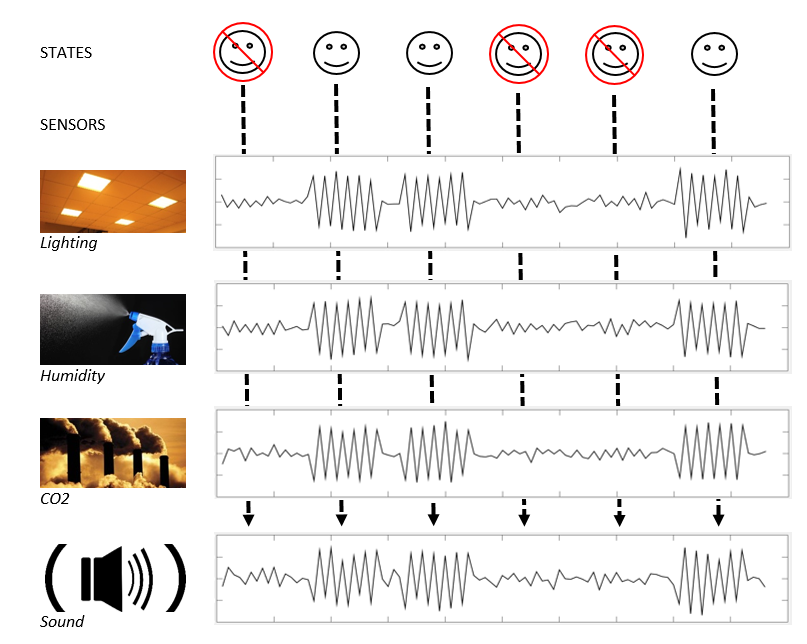
\includegraphics[width=3in]{sensorsignals.png}
	
	\caption{Example of sensor signals that can be used to detect presence/absence of people in buildings.}
	\label{fig5}
\end{figure}



In order to overcome these limitations, we present an  Dynamic HSMM (D-HSMM) algorithm, which extends the concept of an explicit HSMM traditional model. Our npvel aproach consists in of modelling each state using different duration distributions using a continuous density function in addition to a minimum and maximum state duration parameter. Also, we model the observations for each sensors signal separately, to later aggregate all the signals in a weighted fashion to calculate a more realistic emission probability. As a result of combining these ideas, we make D-HSMM capable of performing accurate state prediction using just initially partial data and achieving performance results even beyond than other offline Markov approaches. We evaluate our model using a dataset where binary signals from 14 different sensors are used to model presence and absence states in a domestic scenario.

The rest of this paper is organised as follows: Section 2 gives a comprehensive review of the previous related work, Section 3 defines the theoretical concepts of the techniques we have applied, Section 4 describes how our proposal faces the identified issues, Section 5 presents an experimental evaluation of our model and Section 6 concludes with a discussion about the model performance and future work.

%\begin{figure}[!b]
%	\centering
%	\includegraphics[width=3in]{HSMMstruct.png}
%	
%	\caption{Arrival and departure times (Left). Basic Markovian transition structure (Right).}
%	\label{fig6}
%\end{figure}

\section{Previos Work}
Hidden Markov and semi-Markov techniques have recently been applied in many pattern recognition problems. Occupancy pattern modelling using Markovian models include the early works of Page et al \cite{Page2008} where an stochastic model based o Markov chains was proposed in order to create occupancy profiles in an office building or the work in \cite{Si2005} where an HMM model was used to create context-aware scenarios to regulate different smart-home systems. 

Other models based on HMM extensions also became increasingly popular for occupant behaviour pattern recognition modelling approaches as in \cite{Yamagishi2006}. Hongeng et al.  \cite{Hongeng2004} proposed a video based event recognition where an adaptation of HMM algorithms was used to detect human activities through video data, as well as the authors in \cite{Yamazaki2005} who developed a multi regression hidden semi-Markov model for walking motion modelling though fast video data manually labelled. HSMM models were also presented in \cite{Pavel2006} introducing an elderly care monitoring system or in Doung et al.'s model\cite{Duong2006} which included different duration distribution functions (i.e. Gamma, Poisson or Inverse Gaussian) for activity recognition purposes. 

Most of the approaches described so far claimed that HSMM could outperform the classification accuracies from original HMM approaches with manageable increasing in model complexity and computational costs. That encouraged other inspiring works in the human behaviour pattern recognition field as in \cite{Dong2010b}\cite{Kasteren2011a}\cite{Dong2009a}. Dong's work \cite{Dong2009a} presented an HSMM-based occupancy modelling approach for energy savings and comfort management by detecting events extracted from multiple sensor data. Later, in \cite{Dong2010b} they used HMM and other machine learning approaches to detect occupants in an office building based on multiple ambient sensors, noting that different features (sensors) are potentially more significant for the final state classification decision and that HMM can even be used for predictive purposes. Van Kasteren research \cite{Kasteren2011a} provided an interesting activity recognition benchmark work where HMM and HSMM models were evaluated and compared with other state-of-the-art approaches to study modelling issues and performance based on contextual aspects such as time granularity. 

In spite all the progresses, little works have been devoted to the development of models for real-time occupancy classification tasks using streaming data. One of the causes probably lies in the fact that using of Markov models for online occupancy detection is subject to specific challenges, particularly because of the need of whole offline data sequences to produce accurate state inference. Few approaches have been studied to address these challenges, mostly based on sliding window approaches \cite{Krishnan2014}. Here we present a DHSMM model that is designed to tackle online limitations by adapting observation and duration models to the specific needs for modelling occupancy behaviour pattern datasets in an streaming fashion.



\section{HSMM Model Definition}


Here we outline how Markov models are defined and the challenges they usually face for state classification particularly within our domain. 

Let $S_T$ be a set of states that are present in a dataset with a total number of samples $T$. $M$ would be the total number of different states and each time $t=\{1,2,...,T\}$ represents a time step comprising the whole dataset.

%**************************************************************************************************************
%\begin{figure}[!t]
%\centering
%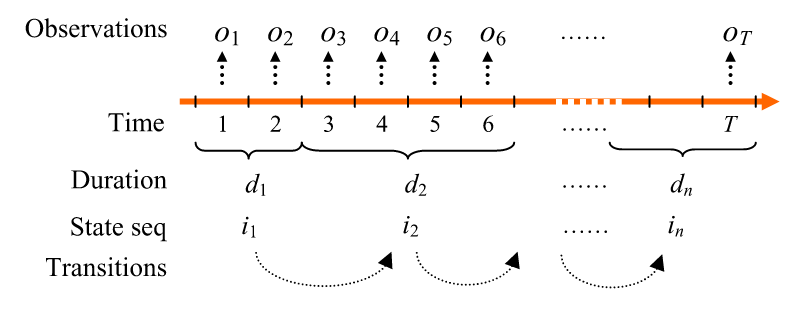
\includegraphics[width=3in]{HSMMGraph.png}
% 
%\caption{HSMM Structure.}
%\label{fig1}
%\end{figure}
As discussed in orevious sections, HMM can only model state duration exponentially. Hidden semi-Markov model was introduced as an extension of the original HMM, where additional parameters were include in order to model durations in a explicit way. HSMM parameters are defined by \begin{gather*} 
\lambda= (Q,O, a, b, \delta, \pi).
 \end{gather*}
 
  Where, $O=\{o_{t}|t \in T\}$ and  $Q=\{q_{t}|t \in T\}$ are the observations and the states respectively for each time $t$.  $a$ represents the $M$x$M$ state transition matrix containing the probability of transitioning from state $i$ to $j$, $a_{i,j}=p([q_t=s_j|q_{t-1}=i])$ represented by:

\begin{centering}
\vspace{0.2cm}
$a_{i,j} = \left( \begin{smallmatrix} a_{1,1}&a_{1,2}&...&a_{1,M}\\ a_{2,1}&a_{2,2}&...&a_{2,M}\\
...&...&...&...\\
a_{M,1}&a_{M,2}&...&a_{M,M} \end{smallmatrix} \right)$
\vspace{0.2cm} 
\end{centering}

Note that, due to the Markovian assumption these models calculate probabilities by looking at the immediate previous state. The emission probability $M$x$N$ matrix $B$ expresses what is the probability $b_{i}(v_i)=p([o_t=v_i|q_{t}=s_i])$ for each state to trigger each of the observations $v_i$, $i=\{1,2,...,k\}$ where $k$ is the number of features. The parameter $\pi$ represents the $M$x$1$ array which contains the prior probability of each state $\pi_i=p([q_{1}=s_i], i=\{1,...,M\})$. 

Finally, duration parameter $\delta$ is the ($M$×$D$) matrix where $D_i$ expresses maximum state duration and $\delta(d)=p(\delta_{s_i}=d)$ is the probability
of state $s_i$ lasting for $d$ time steps. 

Given the above parameters we can express the joint probability of the observations and the hidden states by:

\begin{gather*} 
p(O,S)= \prod_{t=1}^{N}p(O_{t}|S_{t})p(S_{t}|S_{t-1},d_{t-1})p(d_{t}|S_{t},d_{t-1})
\end{gather*}

For the maximisation of this joint probability, several dynamic programming algorithms have been proposed which allow to calculate the most likely state sequence for a given $\{O_T,\lambda\}$, the most likely observation sequence for $\lambda$, or the most probable parameters that maximise $\{S_T\}$. However, these are out of the scope of this work as we will merely calculate probabilities based on immediate new observation points and remaining state duration probabilities. See Rabiner et al. tutorial for  more information about these techniques \cite{Rabiner1989}.

%\subsection{HSMM occupancy inference}
%Occupancy models are frequently used to regulate BMS in real time to adapt the consumption to actual occupant needs. Therefore, it is necessary that these models are able to infer states in 'real time'. Because of the particularities of the semi-Markov models, it is interesting to discuss what differences we might face when performing offline and online inference.
%
%\subsubsection{Offline Inference} 
%In order to perform offline state prediction, Markov models need whole observation sequences. Furthermore to predict state sequences given new observable data, they use recursive (forward-backward) algorithms. These dynamic programming approaches are necessary in order to infer the best state sequence reducing computational costs and complexity. However, they require the whole testing set to be run. 
%
%\subsubsection{Online Inference}
%Contrarily as what happened with the offline example, when performing inference with streaming data we don't have all the training data from the beginning and we can only use one observation at a time. The traditional way to calculate the probability is based on the observation sequence at that time, the model predicts the most probable state and samples a duration value from the $\delta$ distribution. The system then will remain in that state until the duration counter reaches zero in which will transition to another state based on the new observation and the previous state (Markovian property). This presents two major difficulties: 1) when we enter a new state, we don't have all the observation sequence that will come gradually as duration time decreases; 2) as the state duration is also sampled when a new state is entered, this $d$ value will not be flexible and adaptable to the subsequent real input of streaming data.


\section{Proposed Methodology}

In order to make HSMM capable of performing accurate real-time occupancy detection, we present a dynamic hidden semi-Markov approach D-HSMM. Initially, we based our approach in the explicit HMMs which assumes that transitions are independent of the duration of the previous state, self transitions are not allowed ($a_{ii}=0$) and state duration os only dependent on the current state an independent on the previous one\cite{Yu2010}. Our proposed approach extends these traditional explicit models in two main aspects:

\begin{itemize}
	\item We do not establish a boundary for state transition when a new state is reached. Instead, we use a remaining state cumulative probability with \textit{Min\_Dur} and \textit{Max\_Dur} additional parameters.
	\item We infer the new state based only on one initial observation $O_t$, therefore we need to maximise the representativeness of that observed values by computing the likelihood of each separated sensor (one feature per sensor) and we assign a data-driven weight parameter. 
\end{itemize}

%Moreover, in the case of 'live' detection, the systems need to be able to achieve good classification performance using only one new datapoint at a time. As mentioned above, offline inference algorithms have limitations when performing real-time detection. Assuming that we have enough data to initialise the model, the subsequent data will be feed into the model in an streaming fashion meaning that we don't have the whole observation sequences beforehand. Moreover, inference recursive algorithms need the whole sequence to estimate the most probable path given a whole bounded sequence. It is therefore necessary to find a way in which incorporating only one time step at a time the model will still be able to perform state prediction accurately. 
%
%Traditional procedures found in literature for 'live' inference suggest the use of the observation available at some $t$ to make an initial guess and then sample a duration time. This duration value which will start decreasing so the state will not transition until the duration counter reaches 0. This results in a naive approach that don't really capture the dynamics of the occupancy models as it is not expected that the state changes while the counter is still on. We propose a duration modelling approach in which we study the CDF of each state duration rather than only sampling the best duration estimate. We then use this function together with each timestep observation to decide whether we remain in the current state or we move to the next one dynamically. 

\begin{figure}[!t]
	\centering
	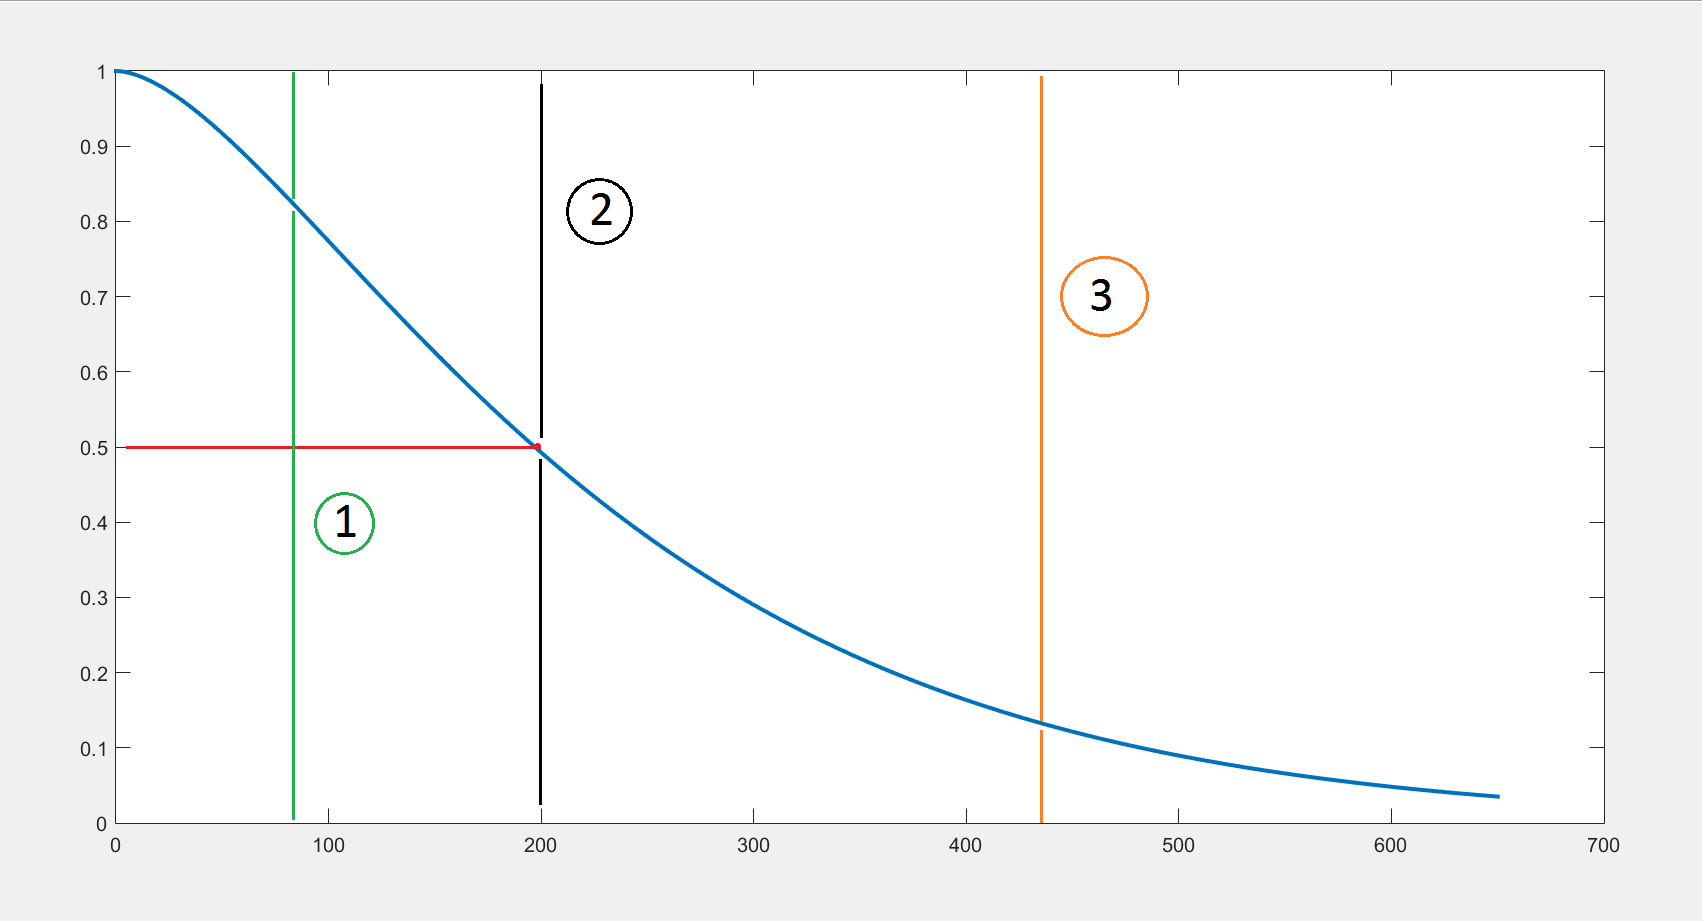
\includegraphics[width=3in]{cdf.png}
	
	\caption{Probability of remaining in the same state (blue) stays during \textit{Min\_Dur}, then decreases based upon the CDF obtained from fitting the data to the duration distribution function that best fits the data. In the unlikely event of reaching \textit{Max\_Dur}, the probability of remaining will equal to 0, forcing the system to abandon the state. For example, in 1) it is likely to remain in the state; in 2) it is equal and in 3) the higher probability is to leave. The final transition event will be chosen by combining duration with observation probabilities.}
	\label{fig2}
\end{figure}

%Our Dynamic hidden semi-Markov model based approach (D-HSMM) enhances the original proposal in order to be able to process streaming data accurately and to be able to adapt to multiple occupancy scenarios introducing weighted features. This new approach is intended to perform real-time occupant presence classification overcoming the traditional online limitations for traditional HSMM approaches. The advantages of D-HSMM can be summarised as follows:
%
%\begin{itemize}
%	\item It allows to make a constant monitoring over the whole state duration by following the duration CDF and calculating the best state probability with the inclusion of each new data point.
%	\item Minimum state duration is included as a new parameter to make duration modelling more realistic.
%	\item Different statistical functions can be used to model each state separately improving model robustness. 
%	\item The sensor inputs used to calculate emission probabilities are incorporated as several normalised inputs rather than a single input sequence. We also include a weighted parameter to each sensor signal in order to capture the differences in the relevance each sensor signal has within the system.
%\end{itemize}

\subsection{D-HSMM duration modelling}
D-HSMM duration model is similar to the work in \cite{Marhasev2006} in which a non stationary time dependant duration HSMM was introduced. Our approach is designed to keep track of the highest state probability each timestep, therefore a transition boundary is not agreed initially by sampling a likely duration when a new state is reached. Instead, we define a CDF function based on different statistical probabilistic functions. The probability of remaining in the same state will remain 1 the number of timesteps specified in the parameter \textit{Min\_Dur}. Consequently, during that period of time, the state will remain unchanged regardless what observations occur. Once \textit{Min\_Dur} has ended, the CDF will decrease according to the probabilistic function and parameters of choice until reaching \textit{Max\_Dur}. During this interval, the combined probability of remaining (extracted from the CDF) and the observation probability ($b_t(O_t)$) will dynamically determine whether to stay in the same state or transition to the next one. Once decided to leave the state, the next observation and the transition probability will be used to determine the most likely new state to enter.

The example in figure \ref{fig2} shows a CDF generated from fitting the data with a gamma distribution. The function has a value of one for the number of timesteps corresponding to the minimum duration parameter (30) and it gradually descends until it reaches a value of zero when $d=D$. This approach also allows the use of the statistical function that better represents the data for each state. In our experiments, we have used a mixture of histogram visual inspection and a MSE error function to choose the best probabilistic function fit for each class (see figure \ref{fig4}).

\subsection{D-HSMM weighted emission parameters}

In the original HSMMs and HMMs, the observation model can be estimated following two approaches: 1) all sensor inputs at a time $t$ can be considered as a unique observation $O_t$ consisting of an array of sensor signals at a determined time, or 2) each sensor signal is assumed to be a different observation but happening at the same time. Therefore, to compute the emission probability in the first case we have the probability of occurring a certain combination of sensor signals whereas in the latter we need to calculate the probability of each of the sensors for a given state. For example, if we want to compute the probability of 3 binary sensors being $Z1=1$, $Z2=1$ and $Z3=0$ at time $t$ given a system with two states $S_i$, i=\{1,2\}, the two options would be: 

1) The probability of the sequence [Z1,Z2,Z3] to be [1,1,0]

\begin{gather*} 
 b_{S_i}(Z1,Z2,Z3)=\\
P(Z1,Z2,Z3|S_i)=\frac{p(sequence=[1,1,0]|S_i)}{\sum_{i}^{ } p(S_i)};\hspace{0.5cm}or
\end{gather*}

2) A different probability for each sensor

\begin{gather*} 
b_{S_i}(Z1,Z2,Z3)=P(Z1,Z2,Z3|S_i)=\\
\frac{p(Z1=1|S_i)+p(Z2=1|S_i)+p(Z3=0|S_i)}{R_t}
\end{gather*}

where $R_t$ is the normalising factor, subject to $\sum_{i}^{ }b_{S_i}=1$\footnote{Note that each sensor probability should be multiplied. However, we use addition instead as we can normalise probabilities for each state to add to 1. By doing this, we can later assign weights to each sensor.}.

The first approach presents an immediate drawback from the point of view of sensor data modelling: if the number of sensors is high and the different discrete possible values they can adopt is also big, the different possible sequences would be dangerously high. For example, in a system with 20 binary (2 possible discrete values) sensors the number of possible different sequences would be $20^2=400$. For the same number of sensors and 4 possible sensor values, $20^4=160000$. This means that each sequence will be likely to happen a very small number running the risk of encountering many new values that never appeared in the training set.

The 2nd approach do not suffer from this. However, this approach unnaturally evens the importance of each sensor when in many applications has been noted that this is not the right modelling approach and some sensors contribute more to the model outputs \cite{Dong2009a}. To overcome this limitation, we have included a weighted factor $cR$ that is applied to each sensor reading: 

\begin{gather*} 
b_{S_i}(Z1,Z2,Z3)=P(Z1,Z2,Z3|S_i)=\\
\frac{cR_1p(Z1=1|S_i)+cR_2p(Z2=1|S_i)+cR_3p(Z3=0|S_i)}{R_t}.
\end{gather*}

For the weights parametrisation, we have used a MSE correlation function applied to the different sensor signals to find which sensors are more correlated to the training labels. We then use these values to a assign a weight to each sensor probability automatically. By doing this, we ensure the emission modelling will adapt realistically to different scenarios with various sensor topologies and sensors of diverse nature. 

%\subsection{3 Stages Presence Detection Algorithm}
%We have included our HSMM approach in a system designed to detect presence and absence in an office environments 24 hours round. Our system combines 3 powerful methodologies to improve the performance of the model by adapting the best approach for each of the stages.
%\subsubsection{Stage 1.-Arrival and Departure Times (Workday)}
%We firstly define the two possible daily periods for worktime Wt as the different times of the day in which the occupants are in working hours (in the office) and the times occupants leave the office to go home or any other places outside work times (off the office). The transitions between these two periods (arrival or departure events) would be determined by the activation of the sensor ($DoorS$)  in the entrance of the space combined with the probability of being in an arrival or departure period (Stage 1) and the probability of a change between presence/absence based on changes in the indoor conditions (Stage 2). Once we have define whether Wt is ‘true’ and therefore someone has started their workday we will use the changes in the ambient conditions (Stage 2) to estimate possible short absences during the day in combination with an explicit duration model to describe how these short absences are distributed in a typical office day. 
%We define Wt as a binary variable {0,1} where Wt=1 when the working period has begun ($ONDay$) and Wt=0 when occupants are just finished their workday. To calculate the probability of being in each state, we need data where arrival and departure times have been annotated. With these times, we create two different distributions for arrival/departure times and we fit a statistical distribution for each of those according to the best fit of the real data. To provide our model with flexibility when modelling these times, we allow our algorithm to use up to 5 different distributions which be evaluated by comparing the MSE and the CDF of samples from the functions obtained and the real arrival/departure times data. 

\begin{figure}[!t]
	\centering
	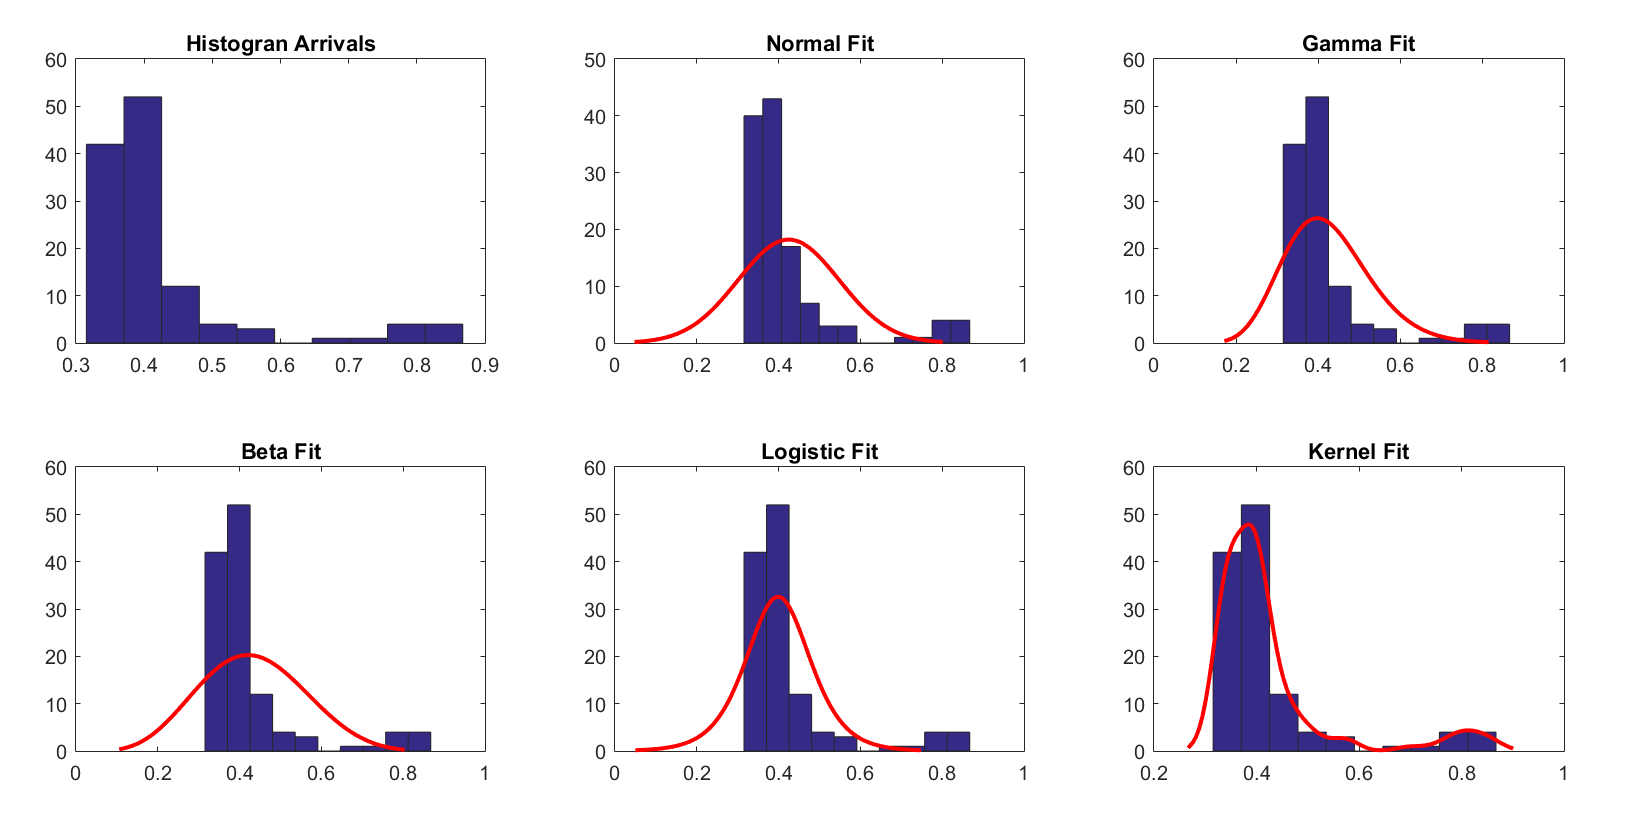
\includegraphics[width=3.5in]{fits.png}
	
	\caption{Functions fitted for Arrival and Departure times.}
	\label{fig4}
\end{figure}

%We define $P(A|ArrivalData)$ as the probability of consider a time of the day as an arrival time based on arrival data and $P(D|DepartureData)$ as the probability of departing at a time of the day. 
%In the Stage 1 of the algorithm, we will be monitoring the state of $Door_S$. $Door_S$ would be a binary variable which will be triggered when someone enters or leaves the office. When $Wt=0$ and $Door_S=1$, the algorithm will compare the current time and calculate the probability of this time being arrival time $P(A)$. This will be especially useful for noise in the data in form of false triggers or in case of other staff checking on the room (i.e. security or cleaning services).  With this information, the algorithm will be in position (using also Stage 2 information) to decide if indeed somebody has started a day in the office; meaning we transition $Wt=0$ to $Wt=1$.

%\subsubsection{Stage 2.-Change Events Detection (SVM)}
%For the Stage 2 of our algorithm we aim to be able to classify when has been a change on the indoor conditions that might indicate a change in the presence/absence state in the room. We define indoor conditions as values the values of temperature, $CO_2$ levels, sound levels or luminance levels. These information will be conditioned by the number of sensors available. It is expected that when somebody enters the office the sensor readings will change accordingly. In the next table we explain what changes might be expected for a series of ambient sensors:
%\begin{table}[]
%	\scriptsize            
%	\centering     
%	\caption{In this table we can see how different sensors might behave in case of an arrival a departure event. Intensity is the proportion of the change in the signal when an event has happened and ratio gives an idea on how much time this changes will be noted by the sensor readings. }
%		\label{my-label}
%	\begin{tabular}{@{}lllll@{}}
%		
%		\toprule
%		Sensor                 & Arrival Event  & Departure Event & IntensIty       & Ratio       \\ \midrule
%		Door Sensor            & Simple Trig. & Simple Trig.  & High            & Immediate   \\
%		Temperature            & Rise           & Drop            & Low/Med     & Slow/Med \\
%		Humidity               & Rise           & Drop            & Low             & Slow/Med \\
%		CO2                    & Rise           & Drop            & Low/Med     & Med     \\
%		Sound                  & Rise           & Drop            & Med/High     & Immediate   \\
%		Appliances & Rise*          & Drop*           & Low/Med/High & Immediate   \\
%		Light                  & Rise*          & Drop*           & High**          & Immediate   \\ \bottomrule
%		
%	\end{tabular}
%\end{table}

%\footnotetext[1]{These readings are likely to be significant for the first arrival/departure of the day. However, in case of short absences no changes might be noted due to leaving for a short while and leaving the lights or the computer turned on.
%\footnotetext[2]{The changes in light levels will be determined by the amount of natural light. In a space with permanent natural light coming it, artificial lights will not be necessary thus the light levels will not change.}
\begin{figure*}[!t]
	\centering
	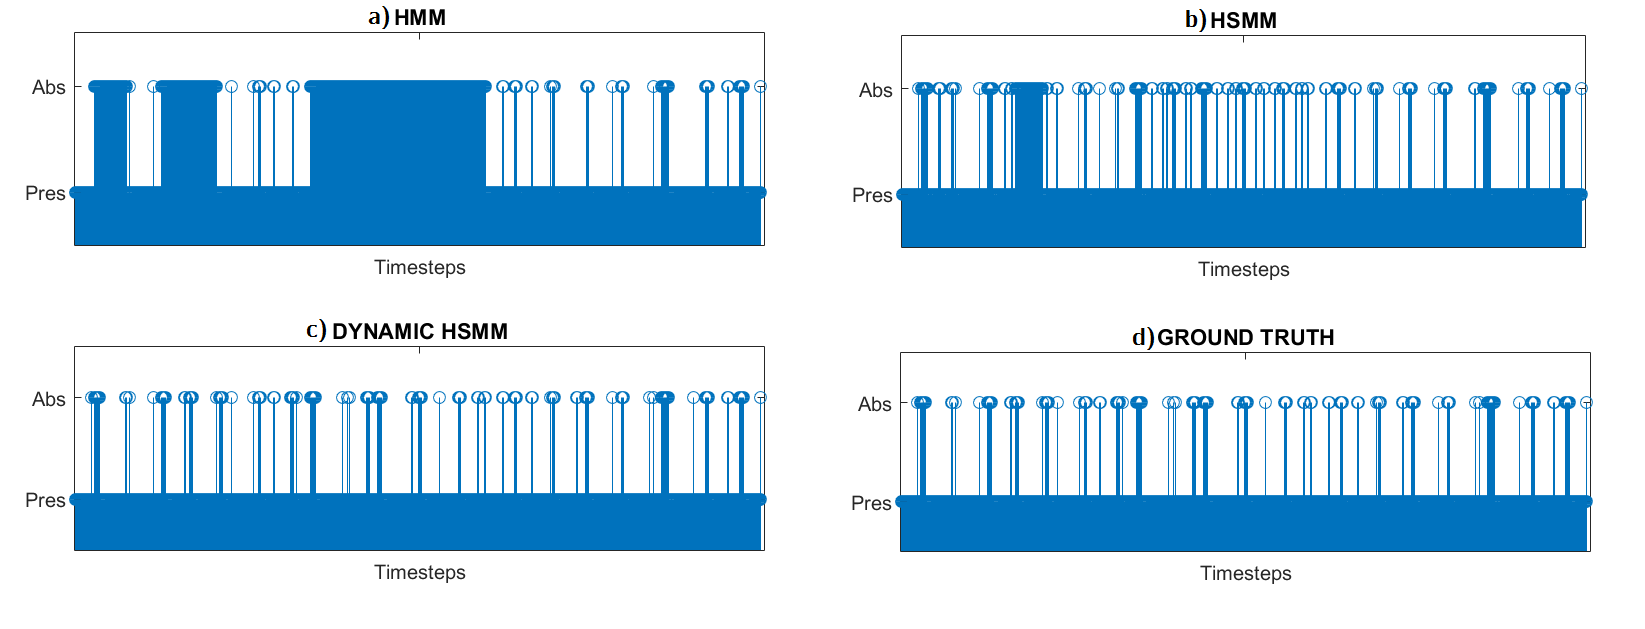
\includegraphics[width=\textwidth]{IMAGES.png}
	
	\caption{Predicted states from HMM, HSMM, D-HSMM against the ground truth.}
	\label{fig3}
\end{figure*}

\begin{figure}[!t]
	\centering
	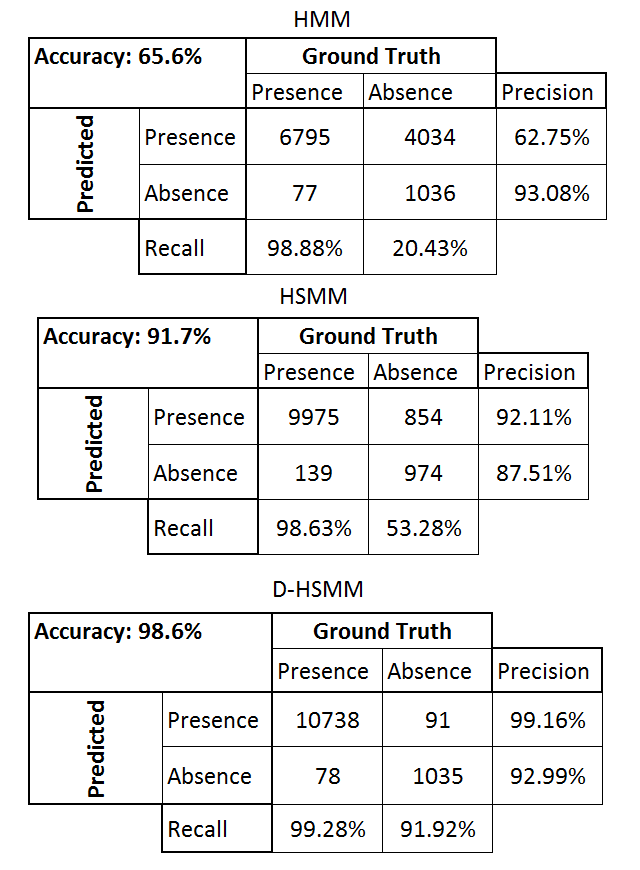
\includegraphics[width=\columnwidth]{confmat2.png}
	
	\caption{Confusion matrices, accuracy, precision and recall.}
	\label{fig6}
\end{figure}

%\begin{figure}[!b]
%	\centering
%	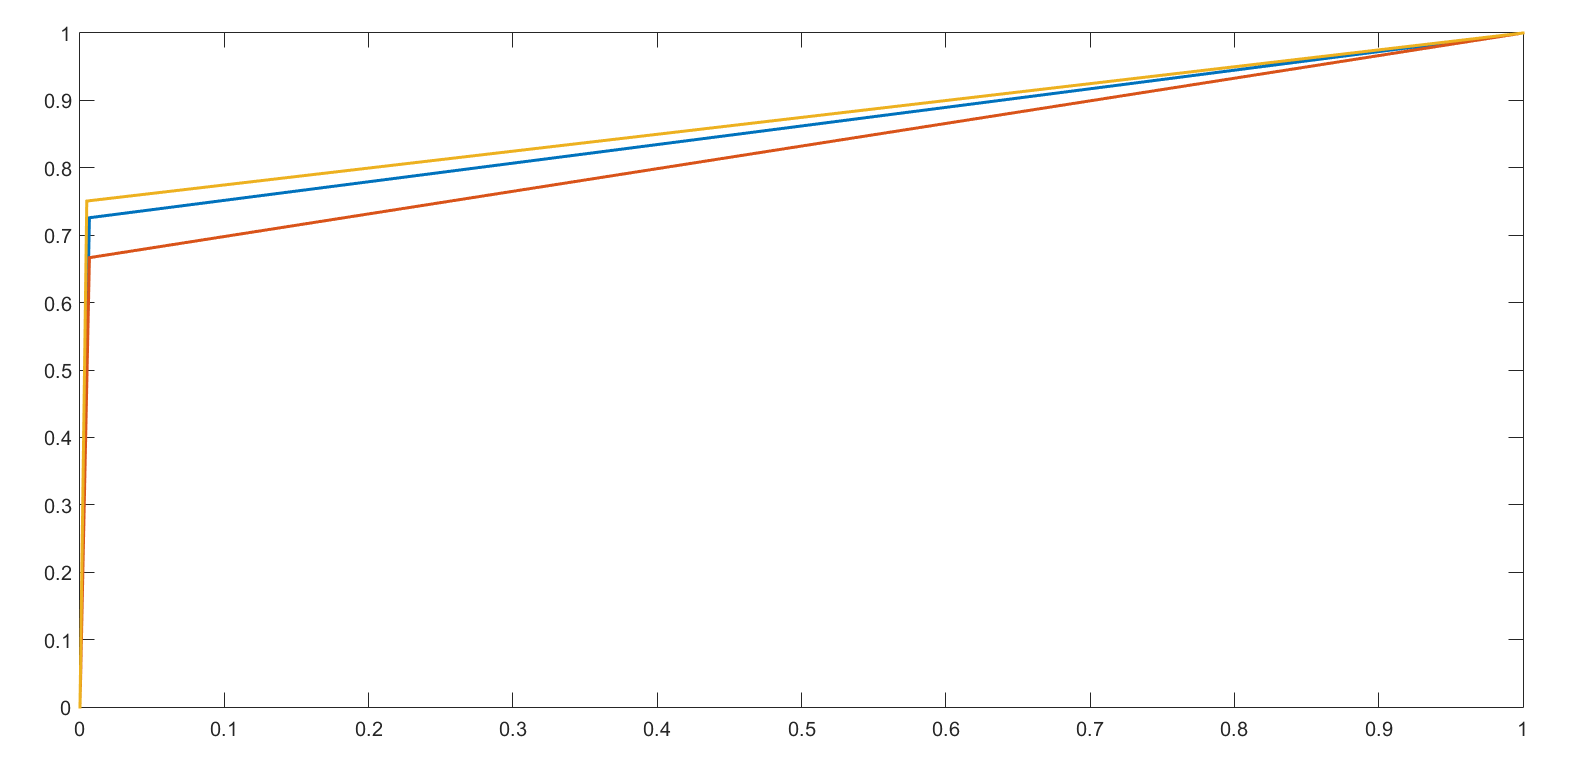
\includegraphics[width=3.5in]{rocCurve.png}
%	
%	\caption{In yellow the D-HSMM ROC curve, blue is HSMM and HMM red corresponds to HMM results.}
%	\label{fig7}
%\end{figure}

%\begin{table*}[]
%	\centering
%	\caption{Confusion matrices}
%	\label{table2}
%	\begin{tabular}{@{}lllllll@{}}
%		\toprule
%		HMM &  &  &  & HSMM &  &  \\ \midrule
%		& Predicted Presence & Predicted Absence &  &  & Predicted Presence & Predicted Absence \\
%		TruePresence & 6275 & 597 &  & TruePresence & 9166 & 948 \\
%		TrueAbsence & 4554 & 516 &  & TrueAbsence & 1663 & 165 \\
%		&  &  &  &  &  &  \\
%		&  &  &  &  &  &  \\\toprule
%		DynamicHSMM &  &  &  & SVM &  &  \\ \midrule
%		& Predicted Presence & Predicted Absence &  &  & Predicted Presence & Predictd Absence \\
%		TruePresence & 10738 & 91 &  & TruePresence & 10716 & 113 \\
%		TrueAbsence & 78 & 1035 &  & TrueAbsence & 53 & 1060 \\ \bottomrule
%	\end{tabular}
%\end{table*}



\section{Experimental evaluation}
We have used sensor data information from a real life scenario for the evaluation of our D-HSMM. From the datasets published in \cite{Kasteren2011a}, we have adapted the data to represent events of people coming in and out from a built environment, therefore the classification task consists of differentiating when the space is occupied or empty. The objective is to prove that D-HSMM is able to perform real-time occupancy classification with high standards of accuracy compared to other state-of-the-art approaches.

\subsection{Data description}
The final data is composed of 2 classes representing presence and absence as our target labels. The observation data consists of 14 different binary sensors (motion, pressure, contact and flush detector). There are a total of approximately 12k labelled samples, each representing an observation sequence of 14 features for each timestep which have been discretised into slices of 60 seconds. 

\subsection{Experimental setup}
We have performed a 3-fold cross validation of the results and we used different metrics to 
validate our results including accuracy, recall, precision and F-score. Each new data point has been processed by our system in a streaming fashion, where predictions have been made without having the whole test sequences. To asses model performance, we have compared our D-HSMM against traditional HMM and HSMM approaches. 

\subsection{Results}
As shown in \ref{fig3} and \ref{fig6}, D-HSMM clearly outperforms the HMM which in most cases fails to reproduce the dynamics of the fast paced short absence periods. Traditional HSMM greatly improves the representation of short periods compared to HMM, however it fails to reproduce sequences with accuracy. Finally, our D-HSMM reaches high accuracy values of over 98\%. 

Other metrics also show D-HSMM performance standards for example recall values for the absence class where HMM and HSMM only reach 20\% and 53\% respectively whereas D-HSMM achieves 92\%. Clearly, results show that D-HSMM significantly outperform original Markov models, both HMM and HSMM and is able to process streaming data with high degrees of accuracy for this dataset. 

 \section{Discussion}
 
 From the experimental results we can conclude that our D-HSMM algorithm achieves the highest levels of classification performance. Our approach improves the HMM and HSMM results using the same data and under the same conditions for all the metrics evaluated. 
 
 Based on these results, it is interesting to discuss why the use of our approach might be beneficial beyond the accuracy figures. Following, we discuss reasons as to why our model is a sound option to better reproduce the real underlying process that theoretically generated the data and why is beneficial when used with real-time data scenarios; frequent in occupancy models.
 
 
\subsection{Generative occupancy models}

% Discriminative models usually have a better overall performance when used to classify complete labelled data without worrying about the process that maps the inputs with the outputs, whereas generative approaches incorporate real insight about the true process as in the case of Markov models that can express the conditional relationships between states and observations and transitions. 
% 
%Discriminative approaches do not try to model the function that originated the data, but simply to find boundaries where the data points exist. That is why they fail to capture the insights and internal complexity of the true function and can be only used to classify between classes. 

Generative models such as HSMMs, can be used to infer states based on new input data and also to create new synthetic data sequences, to retrain model parameters (i.e. the Baum-Welchmann algorithm for Markov models) or to to give further information like the most likely observations given the parameters $\lambda$. Contrarily to the case of the discriminative models, generative ones are intended to approximate the true process that originated the data. Hence their performance tend to suffer when trying to generalise for new data and scenarios. However, D-HSMM not only is capable of modelling occupnacy process but it is also able to perform operation in real time. 
 
 
 
  
 \subsection{Incremental learning}
 Another advantage of HSMMs as well as other Bayesian networks approaches is that they can be adapted to perform incremental online learning; understanding this concept as the update of model parameters alongside the arrival of new data points. These methods usually involve establishing a way of penalising when the model fails to predict a state through a cost function and subsequently. When the system prediction fails, the necessary adjustments in the model parameters are made in order to incorporate the new information without retraining the model from scratch while reducing the rate of failures. 
 
 So far, little researchers have devoted their efforts to the use of semi-Markov models either for streaming data processing or incremental learning. However, current applications increasingly demand these 'live' approaches, therefore it is crucial find ways of adapting our models according to these requirements.
  
 
 \section{Conclussions}
 
 In this paper we have outlined what special requirements a real-time occupancy detection model based upon hidden Markov and semi-Markov approaches need to address in order to accurately detect occupancy behaviour in a variety of scenarios and contextual factors. We have introduced the previous approaches existing and how the traditional methodologies did not take into account the issues to model streaming data using HSMM models. We presented a novel dynamic hidden semi-Markov model D-HSMM algorithm designed to tackle the main issues related to the use of HSMM for 'real-time' occupancy prediction. We have showed how our proposed methodology is able to achieve the highest classification standards compared to previous hidden Markov and semi-Markov models.
 
 \subsection{Future work}
 
We expect to include this algorithm as the final stage of system capable of detecting a whole workday of occupant presence by combining the study of times of arrival/departure though stochastic functions, a change event prediction stage based on a SVM classifier and the final D-HSMM stage which will be in charge of modelling the small periods of absence during a typical working day.
 
 Furthermore, having being able to use a semi-Markov model to perform real-time classification, we can now include an online learning function that will update the model parameters to adapt the system to new unexpected data without having to retrain the model from scratch. Some approaches for the incremental learning of Markov models have already been proposed and the next step would be to include these ideas to further improve our D-HSMM model.
% An example of a floating figure using the graphicx package.
% Note that \label must occur AFTER (or within) \caption.
% For figures, \caption should occur after the \includegraphics.
% Note that IEEEtran v1.7 and later has special internal code that
% is designed to preserve the operation of \label within \caption
% even when the captionsoff option is in effect. However, because
% of issues like this, it may be the safest practice to put all your
% \label just after \caption rather than within \caption{}.
%
% Reminder: the "draftcls" or "draftclsnofoot", not "draft", class
% option should be used if it is desired that the figures are to be
% displayed while in draft mode.
%
%\begin{figure}[!t]
%\centering
%\includegraphics[width=2.5in]{myfigure}
% where an .eps filename suffix will be assumed under latex, 
% and a .pdf suffix will be assumed for pdflatex; or what has been declared
% via \DeclareGraphicsExtensions.
%\caption{Simulation results for the network.}
%\label{fig_sim}
%\end{figure}

% Note that the IEEE typically puts floats only at the top, even when this
% results in a large percentage of a column being occupied by floats.


% An example of a double column floating figure using two subfigures.
% (The subfig.sty package must be loaded for this to work.)
% The subfigure \label commands are set within each subfloat command,
% and the \label for the overall figure must come after \caption.
% \hfil is used as a separator to get equal spacing.
% Watch out that the combined width of all the subfigures on a 
% line do not exceed the text width or a line break will occur.
%
%\begin{figure*}[!t]
%\centering
%\subfloat[Case I]{\includegraphics[width=2.5in]{box}%
%\label{fig_first_case}}
%\hfil

%\subfloat[Case II]{\includegraphics[width=2.5in]{box}%
%\label{fig_second_case}}
%\caption{Simulation results for the network.}
%\label{fig_sim}
%\end{figure*}
%
% Note that often IEEE papers with subfigures do not employ subfigure
% captions (using the optional argument to \subfloat[]), but instead will
% reference/describe all of them (a), (b), etc., within the main caption.
% Be aware that for subfig.sty to generate the (a), (b), etc., subfigure
% labels, the optional argument to \subfloat must be present. If a
% subcaption is not desired, just leave its contents blank,
% e.g., \subfloat[].


% An example of a floating table. Note that, for IEEE style tables, the
% \caption command should come BEFORE the table and, given that table
% captions serve much like titles, are usually capitalized except for words
% such as a, an, and, as, at, but, by, for, in, nor, of, on, or, the, to
% and up, which are usually not capitalized unless they are the first or
% last word of the caption. Table text will default to \footnotesize as
% the IEEE normally uses this smaller font for tables.
% The \label must come after \caption as always.
%
%\begin{table}[!t]
%% increase table row spacing, adjust to taste
%\renewcommand{\arraystretch}{1.3}
% if using array.sty, it might be a good idea to tweak the value of
% \extrarowheight as needed to properly center the text within the cells
%\caption{An Example of a Table}
%\label{table_example}
%\centering
%% Some packages, such as MDW tools, offer better commands for making tables
%% than the plain LaTeX2e tabular which is used here.
%\begin{tabular}{|c||c|}
%\hline
%One & Two\\
%\hline
%Three & Four\\
%\hline
%\end{tabular}
%\end{table}


% Note that the IEEE does not put floats in the very first column
% - or typically anywhere on the first page for that matter. Also,
% in-text middle ("here") positioning is typically not used, but it
% is allowed and encouraged for Computer Society conferences (but
% not Computer Society journals). Most IEEE journals/conferences use
% top floats exclusively. 
% Note that, LaTeX2e, unlike IEEE journals/conferences, places
% footnotes above bottom floats. This can be corrected via the
% \fnbelowfloat command of the stfloats package.







% conference papers do not normally have an appendix


% use section* for acknowledgment





% trigger a \newpage just before the given reference
% number - used to balance the columns on the last page
% adjust value as needed - may need to be readjusted if
% the document is modified later
%\IEEEtriggeratref{8}
% The "triggered" command can be changed if desired:
%\IEEEtriggercmd{\enlargethispage{-5in}}

% references section

% can use a bibliography generated by BibTeX as a .bbl file
% BibTeX documentation can be easily obtained at:
% http://mirror.ctan.org/biblio/bibtex/contrib/doc/
% The IEEEtran BibTeX style support page is at:
% http://www.michaelshell.org/tex/ieeetran/bibtex/
\bibliographystyle{IEEEtran}
% argument is your BibTeX string definitions and bibliography database(s)
\bibliography{biblio2.bib}
%
% <OR> manually copy in the resultant .bbl file
% set second argument of \begin to the number of references
% (used to reserve space for the reference number labels box)
%\begin{thebibliography}{1}
%
%\bibitem{IEEEhowto:kopka}
%H.~Kopka and P.~W. Daly, \emph{A Guide to \LaTeX}, 3rd~ed.\hskip 1em plus
%  0.5em minus 0.4em\relax Harlow, England: Addison-Wesley, 1999.
%
%\end{thebibliography}




% that's all folks
\end{document}


